\subsection{Cross-granularity learning enriches developmental information}
\label{sec:developmental-information}

Having examined the two views in zero-shot tissue mapping, we next ask what cross-granularity learning adds to the retained representations. We compare the final ZoomST and No Cross checkpoints in an equal-budget controlled ablation. No Cross retains within-granularity learning and omits cross-granularity supervision. With both encoders frozen, we evaluate Joint separately at granularities 8, 32, and 128 on held-out MOSTA and HESTA sections, using independently pretrained mouse and human models (Appendix~\ref{app:preprocessing}).

Fine-granularity AMI improves on seven of eight held-out MOSTA sections and all seven HESTA sections (Table~\ref{tab:cross-granularity-ami}a). These AMI gains are modest, prompting us to ask whether the learned relations add information about developmental progression within the same tissue.


We examine Brain through two complementary tasks: developmental ordering and stage prediction. Diffusion pseudotime assesses agreement with the observed developmental sequence through spot-level Spearman correlation. A linear readout tests whether stage can be predicted from frozen representations, training on other sections and evaluating an entire held-out section. Together, these tasks measure unsupervised ordering and the stage information accessible to a supervised readout (Appendix~\ref{app:developmental-ordering}).

The developmental gains are particularly evident in coarse representations (Table~\ref{tab:cross-granularity-development}b). MOSTA shows its largest ordering improvement at the coarsest granularity, where spot-level correlation changes from negative to positive. HESTA shows higher spot-level correlations at every granularity. Stage-prediction error decreases at every granularity in both atlases, with the largest relative MAE reductions at $k=128$: 21.01\% on MOSTA and 8.73\% on HESTA. On MOSTA, adding JointMMD further reduces stage-prediction error relative to CS alone at all three granularities (Appendix~\ref{app:objective-ablation}). Cross-granularity learning thus enriches developmental information within broad tissue contexts, beyond its modest effect on anatomical clustering.

\begin{table}[!htbp]
\centering
\caption{\textbf{Cross-granularity learning across mouse and human atlases.} \textbf{(a)} Joint AMI, with SD over downstream clustering initializations below each mean; sections are averaged equally within each clustering run. Improved counts held-out sections with higher mean AMI. \textbf{(b)} Brain spot-level DPT correlation and leave-one-section-out stage MAE, in embryonic days for MOSTA and Carnegie stages for HESTA. Bold marks the better paired value, including ties. Evaluation protocols: Appendix~\ref{app:dual-view}--\ref{app:developmental-ordering}.}
\label{tab:cross-granularity-ami}
\label{tab:cross-granularity-development}
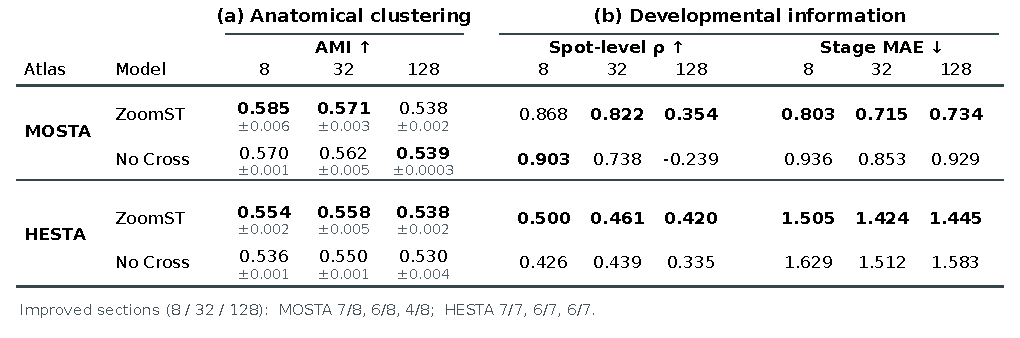
\includegraphics[width=\linewidth]{figures/cross_granularity_combined.pdf}
\end{table}
\FloatBarrier

This developmental information also gives ZoomST an advantage in cross-method comparisons (Figure~\ref{fig:developmental-ordering}). Combining all three granularities, ZoomST achieves the highest spot-level correlation on both MOSTA and HESTA among methods with complete-stage readouts. The ablation and cross-method results show that learning relations across granularities strengthens the developmental content of tissue representations while preserving their anatomical utility.

\begin{figure}[!htbp]
\centering
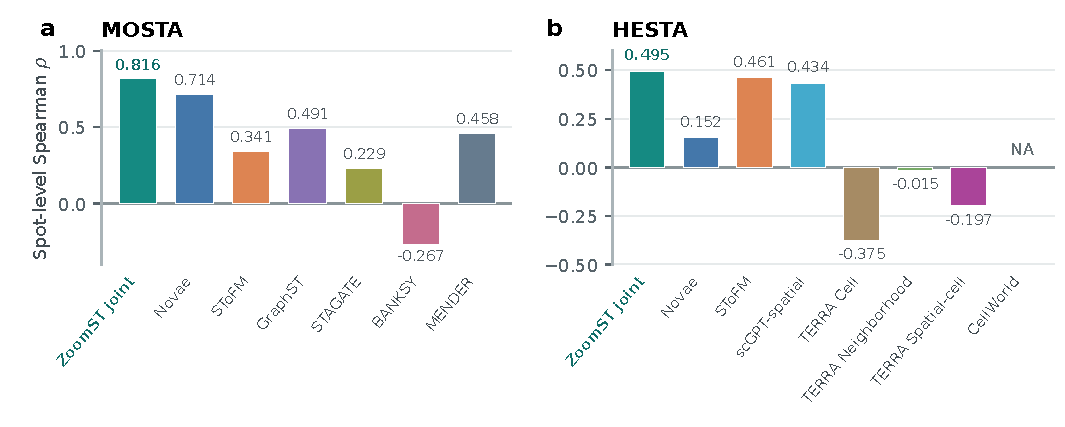
\includegraphics[width=0.98\linewidth]{figures/developmental_ordering_spearman.pdf}
\caption{\textbf{Developmental ordering on MOSTA and HESTA Brain.} Methods share observations and a fixed root within each atlas: (a) MOSTA, 4,712 spots; (b) HESTA, 2,560 spots. ZoomST combines Joint features from three granularities. NA: CellWorld does not connect CS18 to the root. Baseline fitting and DPT settings: Appendix~\ref{app:developmental-ordering}.}
\label{fig:developmental-ordering}
\end{figure}
\FloatBarrier
